\documentclass[../rapport_MVEX01-11-05]{subfiles}
\begin{document}

\section{Klassificering av gester med hjälp av \knn}
Den största andelen korrekt klassificerade gester vi lyckas uppnå
med samtliga gester tillåtna är 91.9\,\%, både med framåturval
och bakåteliminering. Antalet aktiverade
egenskaper blir 10 då algoritmen för framåturval användes och 7 med
bakåteliminering, och antalet närmsta grannar i \knn-metoden är 7. Egenskaperna som
används är listade i
tabell~\vref{tab:bestfeatsfwd}.

Figur~\vref{fig:knn-optimering} visar mer
exakt hur andelen korrekta
klassficeringar beror på antalet aktiverade egenskaper och på värdet av $k$.
Det framgår tydligt att antalet aktiverade egenskaper har stor
inverkan på andelen felklassificerade gester
om man använder sig av färre än
5 egenskaper. Därefter planar andelen ut för att återigen stiga då
fler än 10 egenskaper används. Andelen felklassificeringar
minskar också i takt med att $k$ ökar från 1 till 7, för att sedan
öka då värdet ökar från 7 till 13. Med valet av egenskaper och $k$ tagna från
optimeringen med framåturval presterade metoden enligt
tabell~\vref{tab:tolkningsmatris} och tabell~\vref{tab:prestanda}.

\subsection{Val av egenskaper}\label{sec:resultat_features}
Egenskaperna som använts har visat sig vara mycket bra --- upp till en viss gräns.
I tabell~\vref{tab:bestfeatsfwd} syns de tio egenskaper som inkluderades
med framåturval. Av dessa kan man ta bort tre --- excentricitet,
Hu-moment 2 och Hu-moment 7 ---
med oförändrad klassificeringsförmåga, enligt resultat från bakåteliminering.
De sju bästa egenskaperna som resulterar från
bakåteliminering listas i tabell~\vref{tab:bestfeatsbwd}, i
ordning efter hur länge de är kvar i körningen.

Rankningen av samtliga egenskaper från respektive metod finns i appendix
\ref{sec:egenskapsresultat}.

Ett urval av sex gester visar i
figur~\vref{fig:feats1011} hur de två bästa egenskaperna tydligt samlar 
gesterna i relativt små områden, vilket gör att avstånden i \knn-metoden 
blir mindre. Det ska dock noteras att egenskaperna 
överlappar varandra för vissa gester vilket sannolikt minskar träffsäkerheten.

\subsection{Klassificering i realtid}
Med lämpliga val av egenskaper och en stor, representativ prototypmängd,
kan klassificeraren i realtid klassificera testpersoner, med upprepat
tillfredsställande resultat.

\begin{figure}[p]
  \centering
  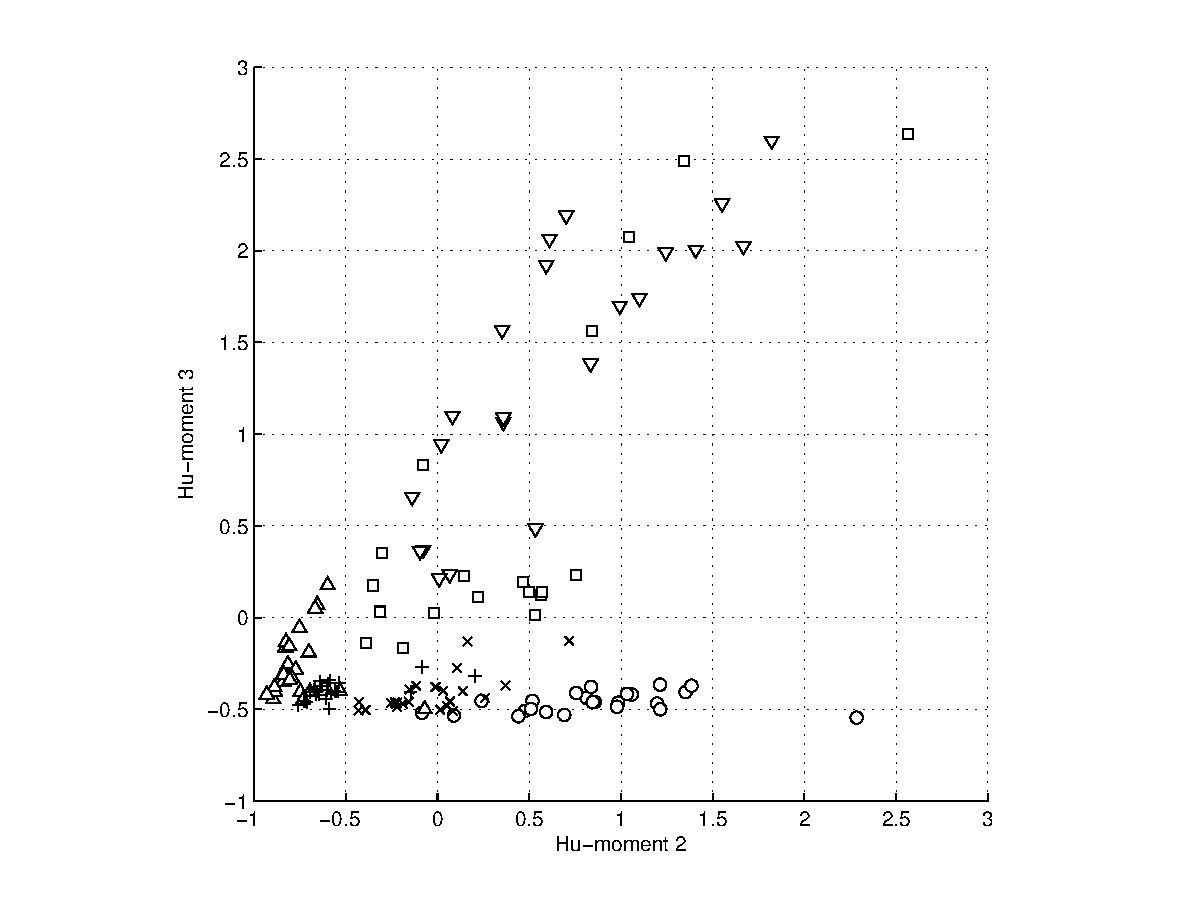
\includegraphics[width=0.75\textwidth,trim=2cm 0.5cm 2cm 0,clip=true]{bilder/feats-10+11}
  \caption{De olika symbolerna motsvarar olika gester, plottade mot de två starkaste egenskaperna
  enligt framåturvalet. Notera hur de flesta är tydligt samlade, men att
	vissa gester överlappar varandra. För två av gesterna (nedåtvända trianglar och fyrkanter) 
	är de två egenskaperna tydligt korrelerade, medan de inte är det för andra.}
  \label{fig:feats1011}
\end{figure}

\begin{figure}[p]
    \begin{center}
        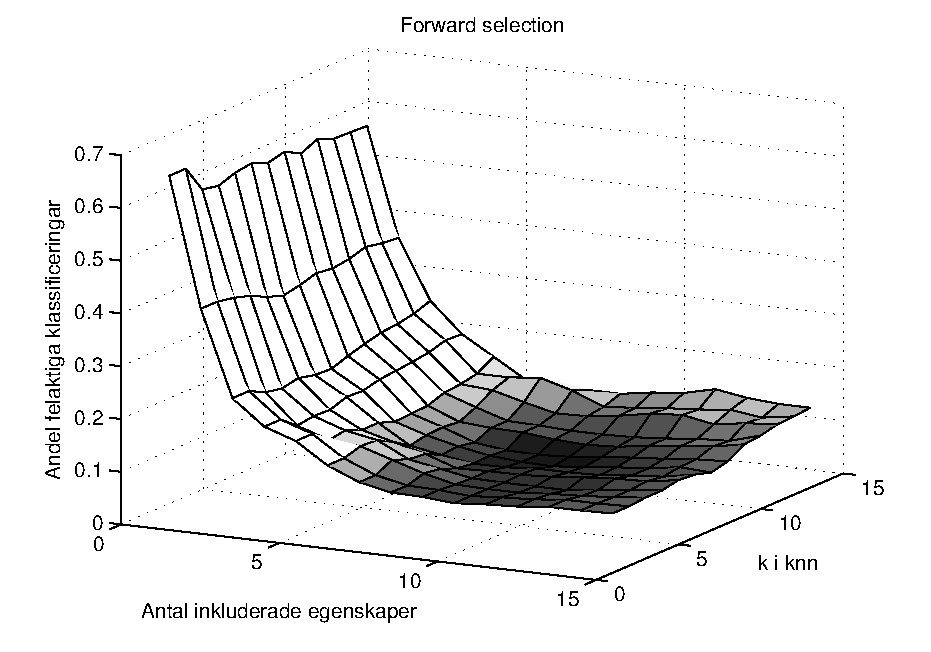
\includegraphics[width=0.75\columnwidth,clip=true]{bilder/fwd_sel}
				%\\\medskip
    \end{center}
    \caption{Optimering av \knn-metoden med avseende på inkluderade egenskaper
och värden på $k$ med algoritmen för framåturval. Ett minimum i
andel felaktiga klassificeringar, 91.4\,\%, fås då
$k=7$ och 10 egenskaper inkluderades. Med bakåteliminering fås
samma minsta andel felaktiga klassificeringar, fast med 7 inkluderade egenskaper
och $k=7$.}
    \label{fig:knn-optimering}
\end{figure}

\clearpage

\begin{table}[p]
	\centering
	\caption{Andel felklassificeringar av statiska gester i procent. Apriorifel
	betecknar sådana fel då gesten varit känd men identifierats
	som något annat; aposteriorifel betecknar sådana fel då
	identifikationen är känd men felaktig.}
	\smallskip
	\label{tab:prestanda}
	\begin{tabular}{c c c}
		\toprule 
		Försöksgest & Apriorifel & Aposteriorifel \\
		\midrule 
		A & 14&15 \\
		B & 11&12 \\
		C & 0& 0\\
		D & 0& 0\\
		E & 30& 41\\
		Sten & 6& 5\\
		Sax & 16& 18\\
		Påse & 9& 9\\
		Spock & 0& 0\\
		Seger & 0& 0\\
		\bottomrule 
	\end{tabular}
\end{table}

\begin{table}[p]
	\centering
	\caption{De tio bästa egenskaperna med framåturval}
	
	\label{tab:bestfeatsfwd}
	\begin{tabular}{ll}
		\toprule
		Rankning & Egenskap \\
		\midrule
		1 & Hu-moment 3 \\
		2 & Hu-moment 2 \\
		3 & Tyngdpunktsläge, $y$-led \\
		4 & Fyrkantighet \\
		5 & Soliditet \\
		6 & Excentricitet \\
		7 & Konvexitet \\
		8 & Hu-moment 1 \\
		9 & Utsträckning \\
		10 & Hu-moment 7 \\
		\bottomrule
	\end{tabular}
\end{table}

\begin{table}[p]
	\centering
    \caption{De sju bästa egenskaperna med bakåteliminering}
       
	\label{tab:bestfeatsbwd}
	\begin{tabular}{ll}
		\toprule
		Rankning & Egenskap \\
		\midrule
                1 & Fyrkantighet \\
                2 & Tyngdpunktsläge, $y$-led \\
                3 & Hu-moment 1\\
                4 & Soliditet\\
                5 & Konvexitet \\
                6 & Utsträckning \\
                7 & Hu-moment 3 \\
		\bottomrule
	\end{tabular}
\end{table}

\clearpage

\begin{table}[p]
	  \centering
		\caption{En s.k.~confusion matrix för klassificering
                  av tio statiska gester. Tecknet för E var det klart
                  svåraste att klassificera, med endast 70\,\%
                  korrekta klassificeringar. Varje gest testades med
                  64 bilder.}
		\label{tab:tolkningsmatris}
    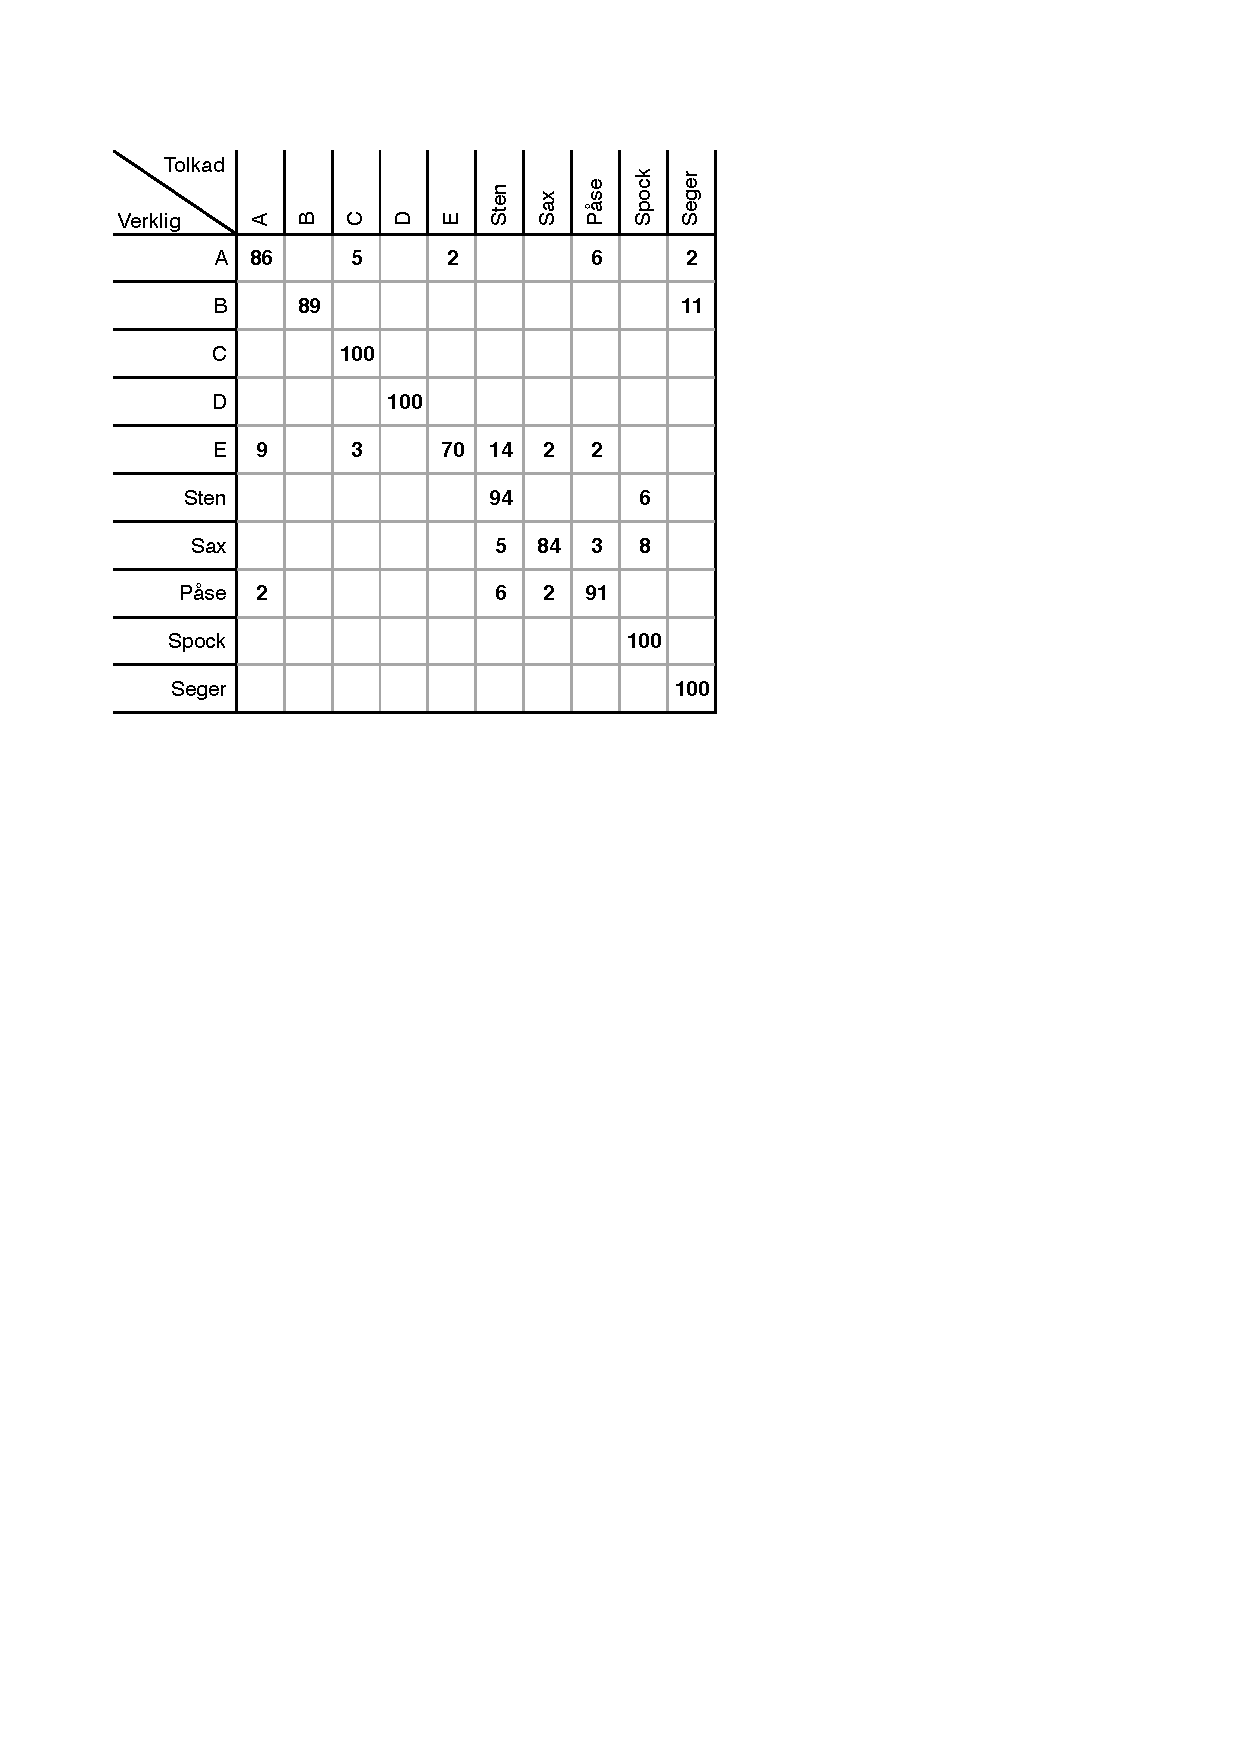
\includegraphics[trim=2cm 16cm 8.875cm
    2.5cm,clip=true,width=0.85\columnwidth]{bilder/tolkningsmatris.pdf}
\end{table}

\end{document}
